\documentclass[10pt,twocolumn, a4paper]{witseiepaper}

\usepackage{KJN}
\hyphenation{op-tical net-works semi-conduc-tor}
\usepackage{graphicx}
\usepackage[export]{adjustbox}
\usepackage{url}
\usepackage{amsmath}
\usepackage{listings}
\usepackage{algpseudocode,algorithm,algorithmicx}
\usepackage{pdflscape}
\usepackage{lipsum}
\usepackage{bookmark}
\usepackage[normalem]{ulem}
\def\code#1{\texttt{#1}}


%----------------------------------------------------------------------------------------
%	PDF INFORMATION
%----------------------------------------------------------------------------------------
\ifpdf
\pdfinfo{
/Title (Project Plan: Image Compression based on Non-Parametric Sampling in Noisy Environments)
/Author (Group 19G01)
/CreationDate (01/07/2019)
/Subject (ELEN4012)
/Keywords (ELEN4012, Laboratory Project, Image Compression, 4th Year)
}
\fi


%%%%%%%%%%%%%%%%%%%%%%%%%%%%%%%%%%%%%%%%%%%%%%%%%%%%%%%%%%%%%%%%%%%%%%%%%%%%%%%
\begin{document}

%----------------------------------------------------------------------------------------
%	TITLE
%----------------------------------------------------------------------------------------

\title{PROJECT PLAN\\ Image Compression based on Non-Parametric Sampling in Noisy Environments}

\author{Group 19G01: Kishan Narotam (717 931) \& Nitesh Nana (720 064)
\thanks{School of Electrical \& Information Engineering, University of the
Witwatersrand, Private Bag 3, 2050, Johannesburg, South Africa}
}


%----------------------------------------------------------------------------------------
%	ABSTRACT
%----------------------------------------------------------------------------------------
\abstract{This report covers the project plan for the laboratory project based on image compression. The project plan looks at the specifications that will define a successful project implementation and a brief look at existing models of image compression. The proposed strategy involves an encoder and decoder side that will be implemented in MATLAB. The encoder side of the strategy involves: reading the image, converting to greyscale, dividing the image into a domain pool, creating holes in the image and compressing the image using known technique. The image is encoded and transmitted through a channel and random errors introduced. The decoder involves: decompressing the image, filling the holes and reconstructing the final image. A performance index is proposed as well as a look into cost management. Time management is discussed in detail with the aid of a Gantt chart and how the documentation of the project will be done.}

\keywords{Image compression, DCT, MATLAB, Project Plan, Hole creation}


\maketitle
%\thispagestyle{empty}
\pagestyle{plain}


%----------------------------------------------------------------------------------------
%	MAIN BODY OF REPORT
%----------------------------------------------------------------------------------------
\section{INTRODUCTION}
\label{sec: Introduction}
A project plan is a formal document that forms a guideline of the project that will ensure the overall success and completion of the project~\cite{Techopedia}. Planning the project involves looking at three fundamental aspects of the project:
\begin{itemize}
\item Scope: what are the objectives of the project and how it will be completed
\item Cost: how much money is allocated, budgeted and spent over the course of the project
\item Time: the time taken to execute the project to a point of completion~\cite{PM}.
\end{itemize}

In the report that follows, a project plan is created for the telecommunications project of \emph{image compression based on non-parametric sampling in noisy environments}. Firstly, the project specifications are defined, followed by a brief look into existing models. Subsequently, the proposed strategy for the project is done with a cost and time management which is discussed in order for the project to be completed on time within a specified budget.

%%%%%%%%%%%%%%%%%%%%%%%%%%%%%%%%%%%%%%%%%%%%%%%%%%%%%%%%%%%%%%%%%%%%%%%%%%%%%%%
%
\section{PROJECT SPECIFICATIONS}
\label{sec: Project Specs}
The aim of the project is to create a robust scheme for determining multiple holes that may be received in an image and appropriately fill these holes. In addition, the image may be subject to random burst errors which need to be identified and corrected.

An image will be chosen for compression utilizing a compression technique and creating holes in the image. After transmission, filling of those holes will result in the original image. The holes will be created manually with a proposed algorithm and the additional compression layer will make use of current compression algorithms (DCT or fractal compression). Once the holes are created, the image will be transmitted via a simple channel that will introduce errors randomly. The image will be received at the receiver, and knowing where the holes are present through the encoding scheme will fill them accordingly using a different algorithm. The receiver will also have to deal with random errors that may have occurred from the channel. The received image with the filled holes will be reconstructed and presented as the final image which should coincide with the original image.

%%%%%%%%%%%%%%%%%%%%%%%%%%%%%%%%%%%%%%%%%%%%%%%%%%%%%%%%%%%%%%%%%%%%%%%%%%%%%%%
%
\begin{figure*}[t!]
\renewcommand{\thefigure}{\arabic{figure}}
\hspace{-0.5cm}
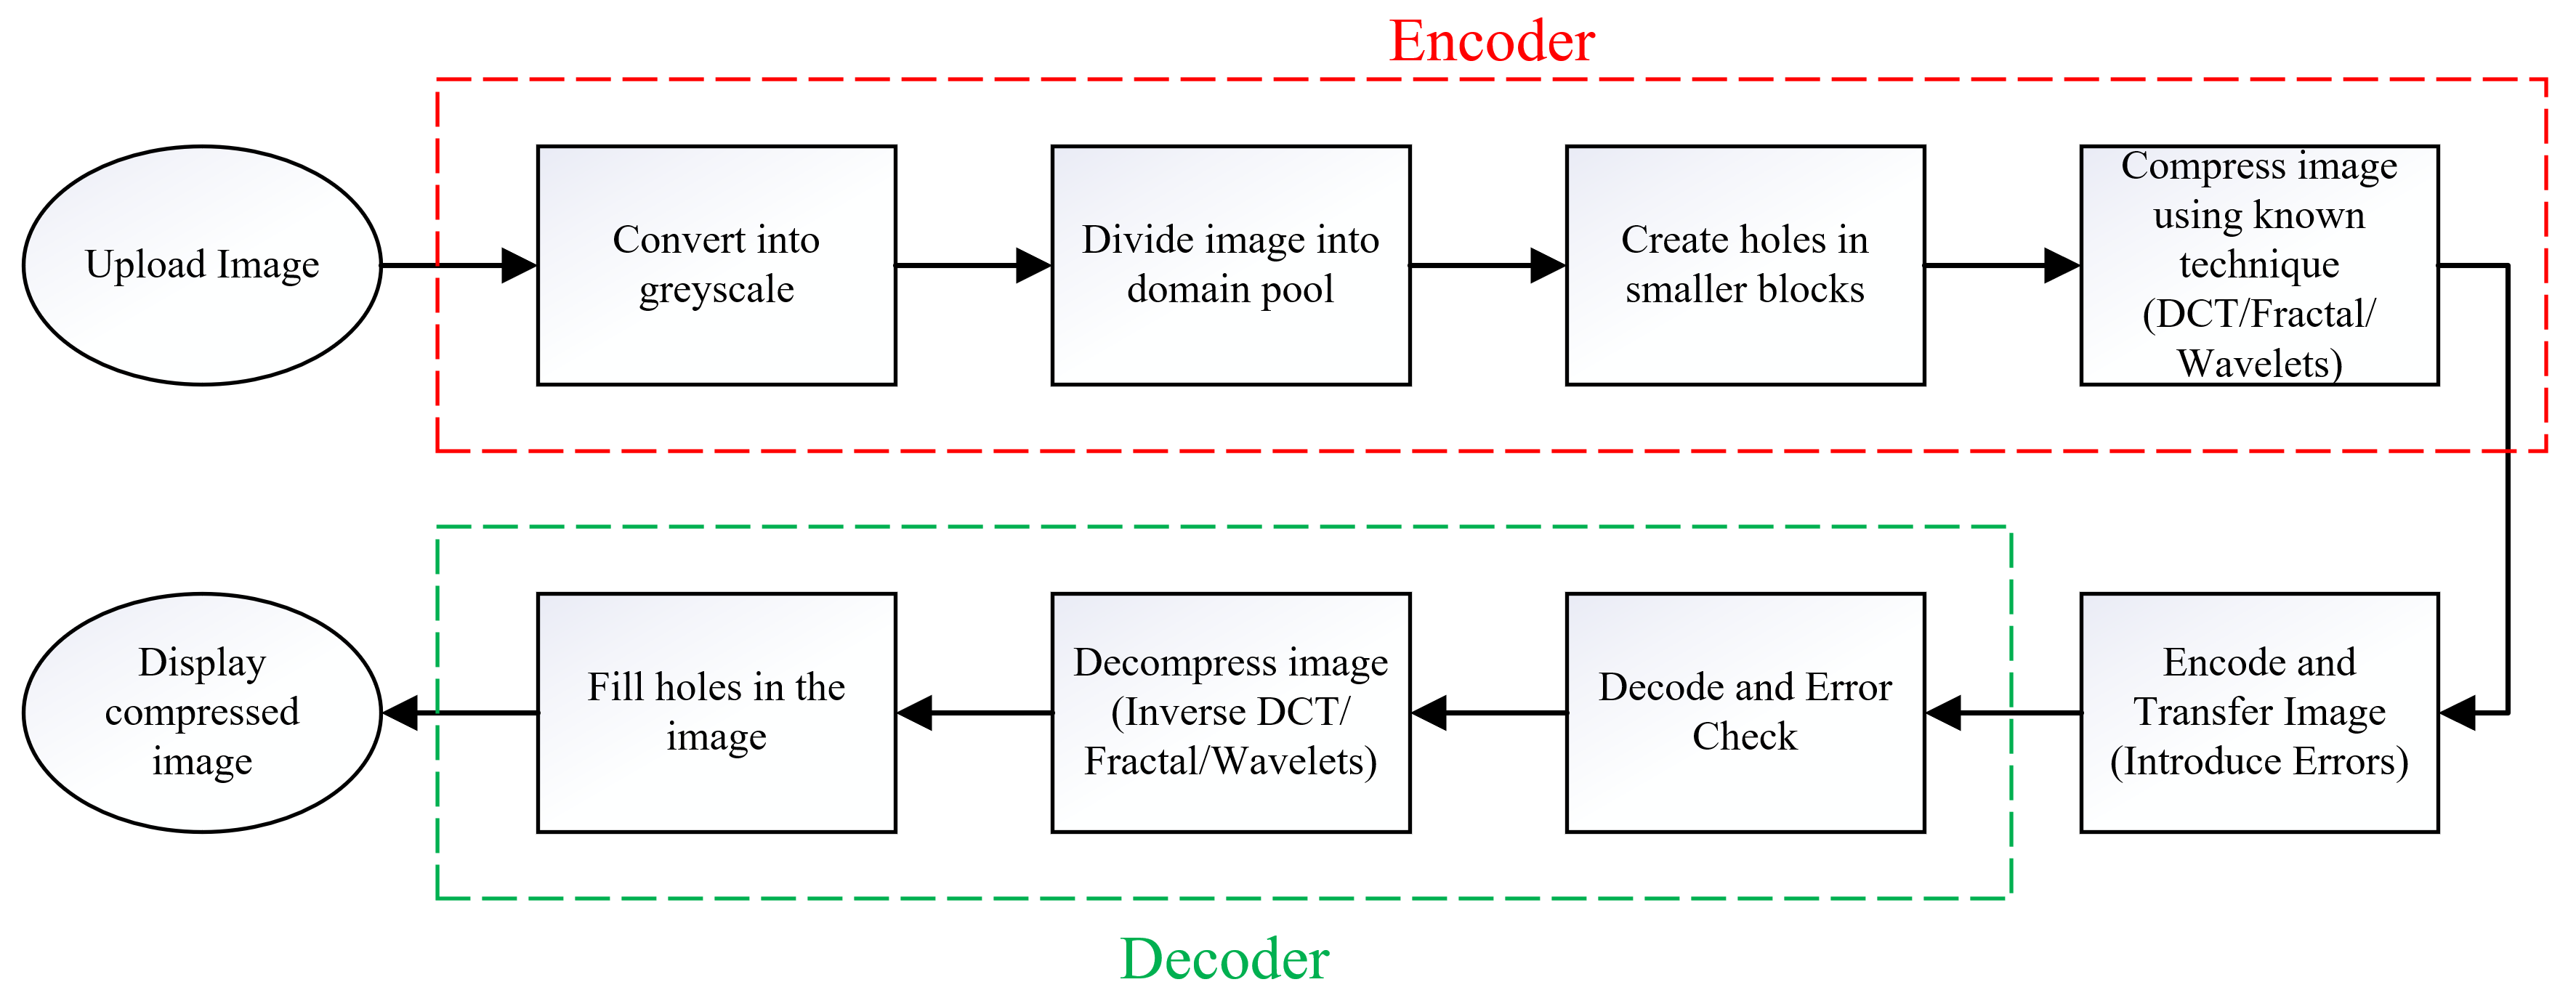
\includegraphics[scale=0.35]{BlockDiagram.png}
\caption{Block diagram of the proposed strategy}
\label{fig: Block Diagram}
\end{figure*}
\section{EXISTING MODELS}
\label{sec: Existing Models}
Image compression is an application of data compression where an image file is encoded with a few bits with the overall goal of reducing the size of the image file compared to that of the original~\cite{ImageComp}. There are two main techniques of image compression:
\begin{itemize}
\item Lossless
\item Lossy
\end{itemize}

\subsection{Lossless}
\label{sec: Lossless}
Lossless compression allows the original form of data to be reproduced, thus meaning that the original data from the file before compression is preserved~\cite{Loss}. Some of the current lossless compression techniques include:
\begin{itemize}
\item Run-Length encoding
\item Huffman encoding
\item Shannon-Fano encoding
\item Arithmetic
\item Dictionary based~\cite{DiffTech}.
\end{itemize}


\subsection{Lossy}
\label{sec: Lossy}
Lossy compression removes some of the data from the original file, resulting in an overall reduction of the size of the file~\cite{Loss}. The non-useful parts of the data that is not noticeable is removed, thus reducing the overall quality of the data and file. Some of the current lossy compression techniques include:
\begin{itemize}
\item Lossy predictive
\item Vector Quantization
\item Transform Coding
\item Block transform
\item DCT/DWT
\item JPEG~\cite{DiffTech}.
\end{itemize}

%%%%%%%%%%%%%%%%%%%%%%%%%%%%%%%%%%%%%%%%%%%%%%%%%%%%%%%%%%%%%%%%%%%%%%%%%%%%%%%
%
\section{PROPOSED STRATEGY}
\label{sec: Proposed Strategy}
The proposed solution will be implemented in MATLAB and can be broken down into two main facets:
\begin{itemize}
\item Encoder side:
\begin{itemize}
	\item Loading/Reading an Image into MATLAB
	\item Converting the image to a greyscale image
	\item Dividing the image into the domain pool
	\item Creating holes in the smaller blocks
	\item Compressing the image using a known technique (DCT/wavelets/fractal)
\end{itemize}
\item Decoder side:
\begin{itemize}
	\item Decode the image and error check
	\item Decompress image (inverse DCT/wavelets/fractal)
	\item Fill holes in the image
\end{itemize}
\end{itemize}
In conjunction with this, a simple channel will be created and random errors will be introduced after the image is encoded. Figure~\ref{fig: Block Diagram} shows the basic framework and block diagram of the proposed solution that will be implemented.

\section{ENCODER SIDE}
\label{sec: Encoder Side}
\subsection{Step 1: Loading/Reading an Image into MATLAB}
\label{sec: Step 1}
Firstly, an image is loaded into MATLAB, and a PNG or BMP image is specifically chosen with the dimensions $M\times N$, where $M$ and $N$ are divisible by 8. A PNG or BMP image is used as a JPEG image, is already a compressed image via the DCT image compression technique. Figure~\ref{fig: Step 1} shows an example of the image that can be used. 
\begin{figure}[h!]
\renewcommand{\thefigure}{\arabic{figure}}
\centering

\includegraphics[scale=0.5, frame]{Step1.png}
\caption{$128\times 128$ image that will be loaded}
\label{fig: Step 1}
\end{figure}

\subsection{Step 2: Convert the image to greyscale}
\label{sec: Step 2}
The loaded image is converted to greyscale. The reason for this is because an image that has been imported into MATLAB creates a 3-dimensional array where the first two elements of the array represent the dimensions of the image and the third dimension is the colour map. Converting the image to a greyscale one, creates a 2-dimensional array, which are simply the dimensions of the image, where each array value correlates to the specific integer value of that specific pixel. Figure~\ref{fig: Step 2} shows an example of the outcome of converting the image to greyscale.
\begin{figure}[h!]
\renewcommand{\thefigure}{\arabic{figure}}
\centering

\includegraphics[scale=0.5, frame]{Step2.png}
\caption{Image after it has been greyscaled in MATLAB}
\label{fig: Step 2}
\end{figure}

\subsection{Step 3: Divide the image into the domain pool}
\label{sec: Step 3}
The image is now divided into smaller $8\times 8$ blocks, creating the domain pool. Once the image has been divided into smaller blocks, we index each block from the top left starting from 1 and increment each index by one, moving left-to-right, top-to-bottom. The reason for creating such an index is so that the receiver will be able to determine which smaller block in the domain pool contains holes so that the receiver can fill these holes. Figure~\ref{fig: Step 3} shows an example of the loaded image having a domain pool of $256$ blocks.
\begin{figure}[h!]
\renewcommand{\thefigure}{\arabic{figure}}
\centering

\includegraphics[scale=0.7, frame]{Step3.jpg}
\caption{Smaller $8\times 8$ blocks creating the domain pool}
\label{fig: Step 3}
\end{figure}

\subsubsection{Indexing the blocks}
\label{sec: Index Block}
Since the images that will be chosen will have dimensions divisible by 8, the first step in determining how many blocks in the domain pool will be created, would be to divide the width and height of the image by 8 to determine how many blocks there will be going across and down the image. Algorithm~\ref{alg: Block index} shows a very high-level approach to finding the top left pixel of a block in the domain pool

\begin{algorithm}[h!]
\caption{High level algorithm of finding the \code{x,y} coordinates of the respective blocks in the domain pool}
\label{alg: Block index}
\begin{algorithmic}
\State \code{xBlocks} $\leftarrow$ \code{widthOfImage/8}
\State \code{yBlocks} $\leftarrow$ \code{heightOfImage/8}
\State Set initial \code{(x, y)} values to be \code{(1, 1)} for block 1
\State To move onto next block:
\State \quad set \code{x} to $8(i)-7$, where $i$ is the block number
\If{\code{BlockNumber > xBlocks}}
	\State Set \code{y} to $8(i+1)-7$
	\State Reset \code{x} to be 1 and move to next block
\EndIf
\end{algorithmic}
\end{algorithm}

\subsection{Step 4: Create holes in the smaller blocks}
\label{sec: Step 4}
With the domain pool created, holes are created by starting at the center square within the $8\times 8$ block. Starting off with the center $2\times 2$ square, the average value of those 4 pixels are calculated. Each pixel in the $2\times 2$ square is compared to the average value of the smaller square using the Chebyshev distance. The Chebyshev distance between each pixel and the average forms the basis of the similarity index that will be used in the project and its implementation. If the value of the similarity index is less than $5$ for all pixels, a hole can be created in those 4 pixels. A larger square in the same $8\times 8$ block is checked with a size of $4\times 4$. The average of these pixels are calculated and as before compared to each value of the center square. This can continue until we reach a center square size of $6\times 6$, which we will define as the largest hole that can be inserted. Algorithm~\ref{alg: Creating Holes} shows a high-level algorithm for creating the holes in the blocks in the domain pool.

\begin{figure}[h!]
\renewcommand{\thefigure}{\arabic{figure}}
\centering
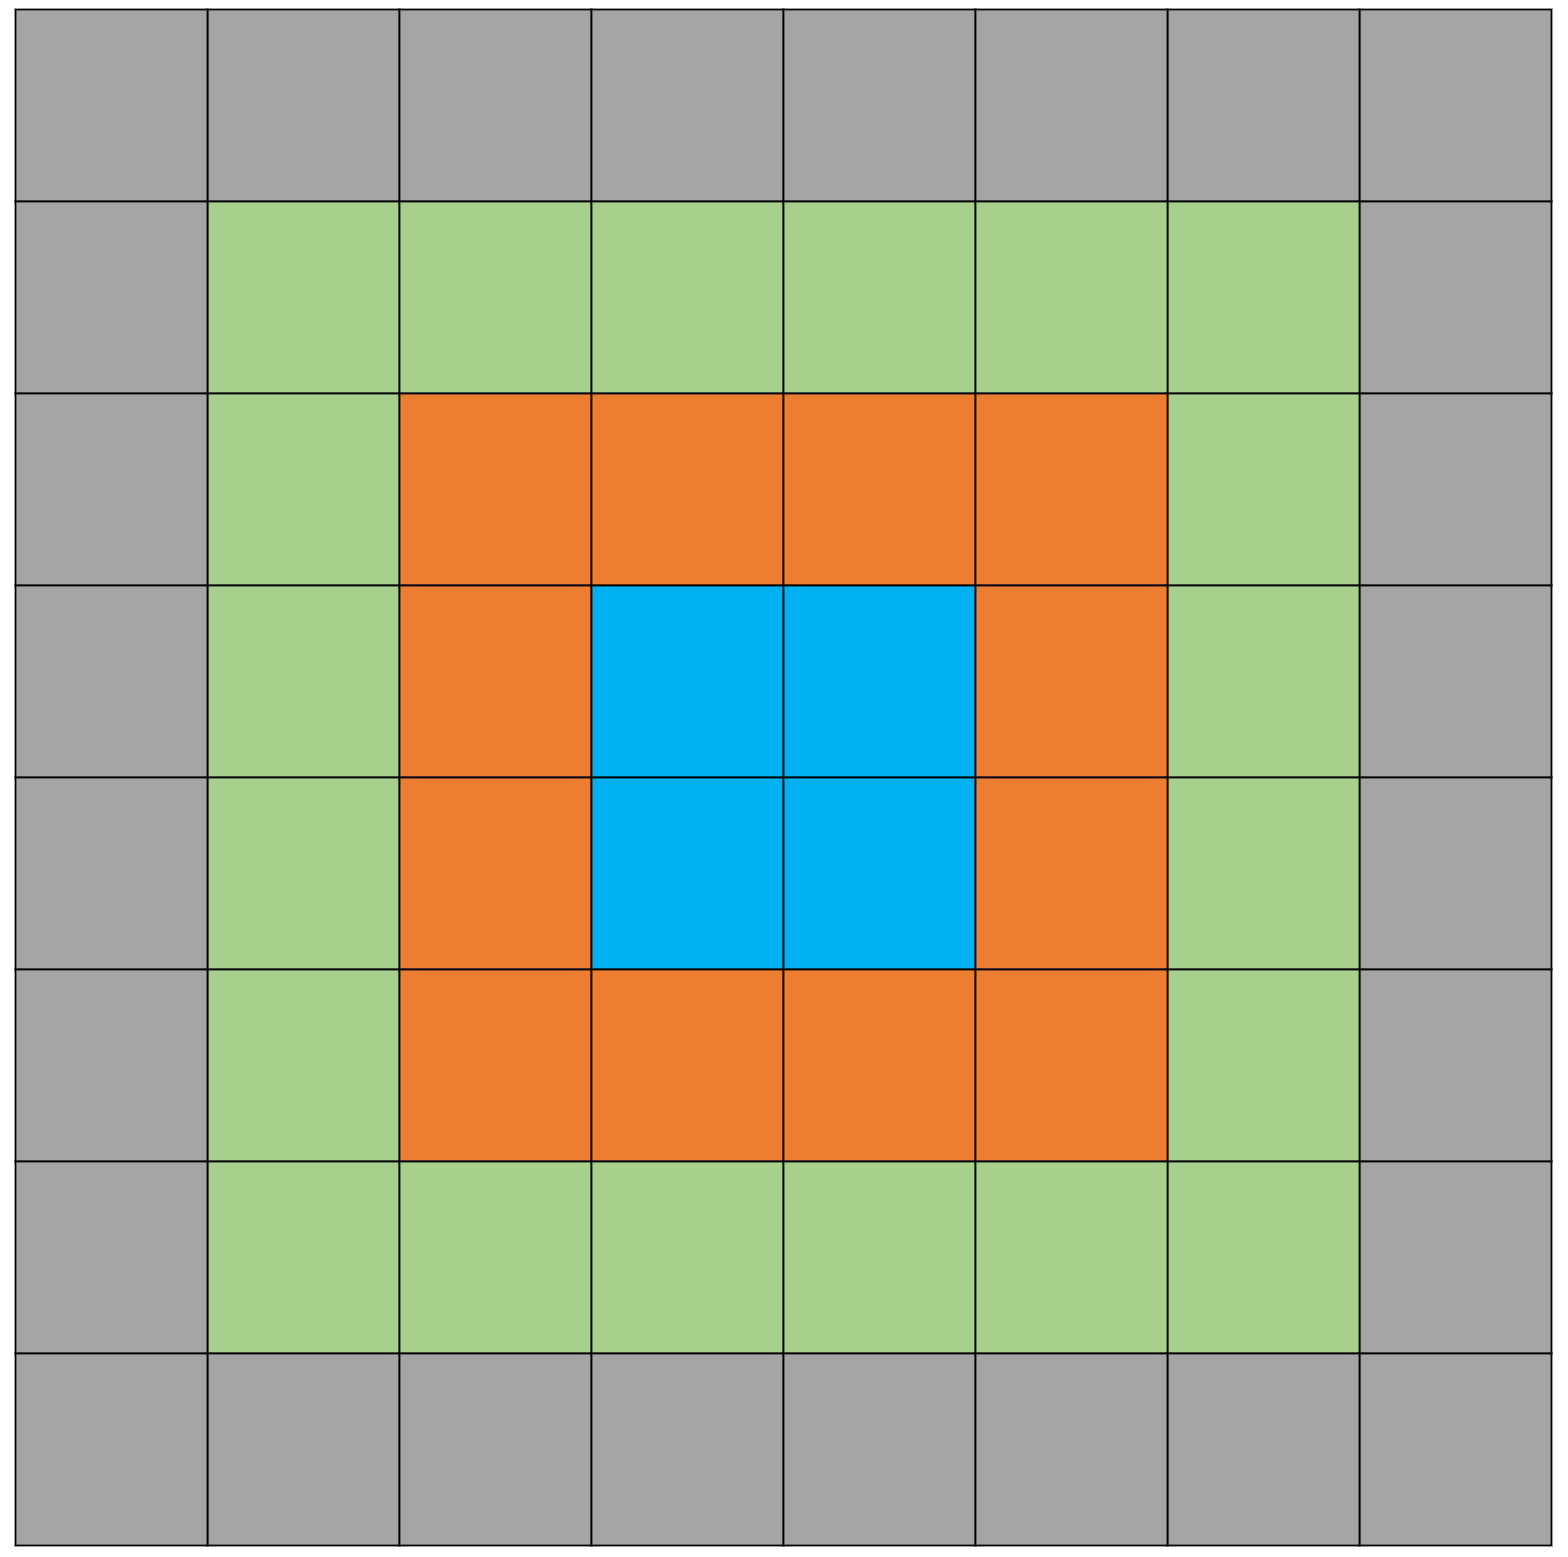
\includegraphics[scale=0.2]{Grid.png}
\caption{How a $8\times 8$ block (grey square) will be checked for hole creation starting with the blue square.}
\label{fig: Grid}
\end{figure}

Figure~\ref{fig: Grid} shows how each of the $8\times 8$ squares in the domain pool, will be checked, starting with the blue squares, moving up to the orange squares to the largest defined hole which are the green squares.

\begin{algorithm}[h!]
\caption{High level algorithm of method of creating holes}
\label{alg: Creating Holes}
\begin{algorithmic}
\State \code{x} coordinate  $\leftarrow$ \code{x+3}
\State \code{y} coordinate  $\leftarrow$ \code{y+3}
\State Calculate average of squares: \code{(x,y; x+1,y; x, y+1; x+1, y+1)}
\For{\code{x} till \code{x+1}}
	\For{\code{y} till \code{y+1}}
		\State Check \code{Chebyshev} distance between \code{(x,y)} and average
	\EndFor
\EndFor
\If{Chebyshev distance between average \& each pixel $\leq$ 5}
	\State Set value in pixels \code{(x,y; x+1,y; x, y+1; x+1, y+1)} to \code{0}
\Else
	\State Compress image
\EndIf
\State
\State \code{x} coordinate  $\leftarrow$ \code{x+2}
\State \code{y} coordinate  $\leftarrow$ \code{y+2}
\State Calculate average of squares (now $4\times 4$ square)
\For{\code{x} till \code{x+3}}
	\For{\code{y} till \code{y+3}}
		\State Check \code{Chebyshev} distance between \code{(x,y)} and average
	\EndFor
\EndFor
\If{Chebyshev distance between average \& each pixel $\leq$ 5}
	\State Set value in pixels to \code{0}
\Else
	\State Compress image
\EndIf
\State
\State \code{x} coordinate  $\leftarrow$ \code{x+1}
\State \code{y} coordinate  $\leftarrow$ \code{y+1}
\State Calculate average of squares (now $6\times 6$ square)
\For{\code{x} till \code{x+3}}
	\For{\code{y} till \code{y+3}}
		\State Check \code{Chebyshev} distance between \code{(x,y)} and average
	\EndFor
\EndFor
\If{Chebyshev distance between average \& each pixel $\leq$ 5}
	\State Set value in pixels to \code{0}
\Else
	\State Compress image
\EndIf
\State Compress image
\end{algorithmic}
\end{algorithm}


\subsection{Step 5: Compress image using a known technique (DCT/Fractal/Wavelets)}
\label{sec: Step 5}
The DCT compression technique will be utilized for the compression of the image. DCT will be performed on each block in the domain pool. DCT is implemented on a $8\times 8$ matrix, which is the reason the domain pool is made up of multiple $8\times 8$ blocks and that an image where the dimensions are divisible by 8 is chosen. The image is now compressed and can be transmitted via the channel. MATLAB has a function built-in to perform the transform, however Equation~\ref{eqn: DCT} shows the mathematical representation of the transform. Fractal or wavelet transformation will be utilized 

\begin{equation}
\label{eqn: DCT}
\begin{split}
D(i,j) =& \frac{1}{\sqrt{2N}}C(i)C(j)\sum_{x=0}^{N-1}\sum_{y=0}^{N-1}p(x,y)\\
& \cos \bigg[ {\frac{(2x+1)i\pi}{2N}}\bigg]\cos \bigg[{\frac{(2y+1)j\pi}{2N}}\bigg]
\end{split}
\end{equation}

\subsection{Step 6: Encode and Transfer image}
\label{sec: Step 6}
The image is encoded as a binary message, and when transmitted through the channel, errors are randomly introduced. The data that will be sent through the channel will be a bit stream and the errors introduced will be based off of a byte with a probability of $10^{-3}$ where the byte can then be randomized. Alternatively each bit can be randomly selected, using the same probability above, to be prone to an error and the bit value flipped.


\section{DECODER SIDE}
\label{sec: Decoder Side}
\subsection{Step 7: Decode and Error Check}
\label{sec: Step 7}
Identification of the location of the errors is required. First, identifying the errors are required, and if detected must be corrected and then the image can be decoded. The image will be converted from a bit stream into its 2-dimensional matrix.

\subsection{Step 8: Decompress (Inverse DCT/Fractal/Wavelets)}
\label{sec: Step 8}
Since DCT compression was used, we now perform the inverse DCT to obtain the compressed image and its respective values in the 2-dimensional matrix.

\subsection{Step 9: Fill holes in the image}
\label{sec: Step 9}
With the one-dimensional array sent across the channel, the blocks within the domain pool that contain the holes can be identified. Starting at outer pixels, the average pixel value of the square is calculated, and that will fill the inner pixels where the hole was created.

%%%%%%%%%%%%%%%%%%%%%%%%%%%%%%%%%%%%%%%%%%%%%%%%%%%%%%%%%%%%%%%%%%%%%%%%%%%%%%%
%
\section{PERFORMANCE INDEX}
\label{sec: Performance Index}
The nature of this project is based around current methodologies and is more research-based. Results are required to present the overall performance of the proposed technique. MATLAB allows for relative simplicity in creating and performing many image compression techniques such as DCT. For that reason, other compression techniques such as fractal compression or wavelets compression will be implemented in addition to DCT compression. The DCT compression will be set as the benchmark and a comparison with the fractal or wavelets compression will be completed. The values of signal-to-quantization-noise ratio (SQNR), peak-signal-to-noise-ratio (PSNR) and mean-squared-error (MSE) will be the main focus of comparison.

%%%%%%%%%%%%%%%%%%%%%%%%%%%%%%%%%%%%%%%%%%%%%%%%%%%%%%%%%%%%%%%%%%%%%%%%%%%%%%%
%
\section{COST MANAGEMENT}
\label{sec: Cost Management}
The nature of this project is software based, and thus the total costs are minimal to none. Licences for the MATLAB software is already provided in the form of a student licence by the university, and personal computers or laptops will be used.

%%%%%%%%%%%%%%%%%%%%%%%%%%%%%%%%%%%%%%%%%%%%%%%%%%%%%%%%%%%%%%%%%%%%%%%%%%%%%%%
%
\section{TIME MANAGEMENT}
\label{sec: Time Management}
The Project window runs from 01 July 2019 until 11 September 2019. The proposed timeline of events and duration of these events can be seen in Figure~\ref{fig: Tasks}, in conjunction with this, Figure~\ref{fig: Gantt} shows the . The project begins with the planning phase including a literature review and the development of the project plan. The overall idea and method was continuously discussed between the team of engineers and the associated supervisor. Once the project plan is approved, the engineers can begin with the execution of the plan.

The encoder side is tackled first while the channel can be created in parallel with that. Once the encoder and channel have been completed and tested, the decoder side of the proposed solution can be implemented. The initial implementation of the encoder will utilize DCT, and once an entire solution is created and tested using DCT, other compression techniques can be implemented in conjunction with the proposed solution. The results of the DCT compression is compared to the other implemented compression technique.

Based on the planned approximated time that is allocated to each task, this indicates that keeping to a tight schedule is required. Since the supervisor will not be available during the first two weeks, the engineers will have to work together and communicate efficiently in order for them to encounter minimal problems and build the proposed solution.

%%%%%%%%%%%%%%%%%%%%%%%%%%%%%%%%%%%%%%%%%%%%%%%%%%%%%%%%%%%%%%%%%%%%%%%%%%%%%%%
%
\section{DOCUMENTATION}
\label{sec: Documentation}
Throughout the project window, constant meetings and discussions will be held between the engineers and the supervisor. As seen in Figure~\ref{fig: Tasks} and~\ref{fig: Gantt} the \emph{Monitoring and Control} task is run from the day after the project plan is submitted till the project is presented. All meetings have and will be documented as meeting minutes, discussing the meeting and the agenda of the project at that period of time. A GitHub repository is created so that the engineers can constantly work on the proposed strategy while keeping all documents and helpful materials available to them at all times.

%%%%%%%%%%%%%%%%%%%%%%%%%%%%%%%%%%%%%%%%%%%%%%%%%%%%%%%%%%%%%%%%%%%%%%%%%%%%%%%
%
\section{CONCLUSION}
\label{sec: Conclusion}
The proposed project plan was given approval by the supervisor. This document discussed existing models of image compression, and gives a detailed description of the proposed strategy of image compression for this project. Block diagrams, example images and high-level algorithms are given as a way of explaining the proposed strategy in more detail. Multiple image compression techniques will be utilized, and the results will be discussed as a performance index. The cost management is discussed, however since the project is research and software-based, no costs will be incurred in the proposed solution. The time management of the project is discussed in detail with a Gantt chart presented as supporting material.

%%%%%%%%%%%%%%%%%%%%%%%%%%%%%%%%%%%%%%%%%%%%%%%%%%%%%%%%%%%%%%%%%%%%%%%%%%%%%%%
%
\begin{thebibliography}{}

%**************************Section**************************%

\bibitem{Techopedia}
Techopedia; \emph{What is a Project Plan? - Definition from Techopedia}; \url{https://www.techopedia.com/definition/24775/project-plan}; Last Accessed: 02/07/2019

\bibitem{PM}
Heerkins, G R; \emph{Project Management}; McGraw-Hill; New York, NY, United States; 1st Edition, 2001

\bibitem{ImageComp}
Wei-Yi Wei; \emph{An Introduction to Image Compression}; Graduate Institute of Communication Engineering; National Taiwan University; Taipei, Taiwan, ROC

\bibitem{Loss}
Chapman, C; \emph{Everything You Need to Know About Image Compression | The JotForm Blog}; \url{https://www.jotform.com/blog/everything-you-need-to-know-about-image-compression/}; Last Accessed: 02/07/2019

\bibitem{DiffTech}
Singh, M; Kumar, S; Chouhan, SS; Shrivastava, M (PhD); \emph{Various Image Compression Techniques: Lossy and Lossless}; Journal of International Journal of Computer Applications; Volume 142; Issue No. 6; pp 23 - 26; May 2016

\end{thebibliography}

\onecolumn
\begin{figure}[h!]
\renewcommand{\thefigure}{\arabic{figure}}
\centering
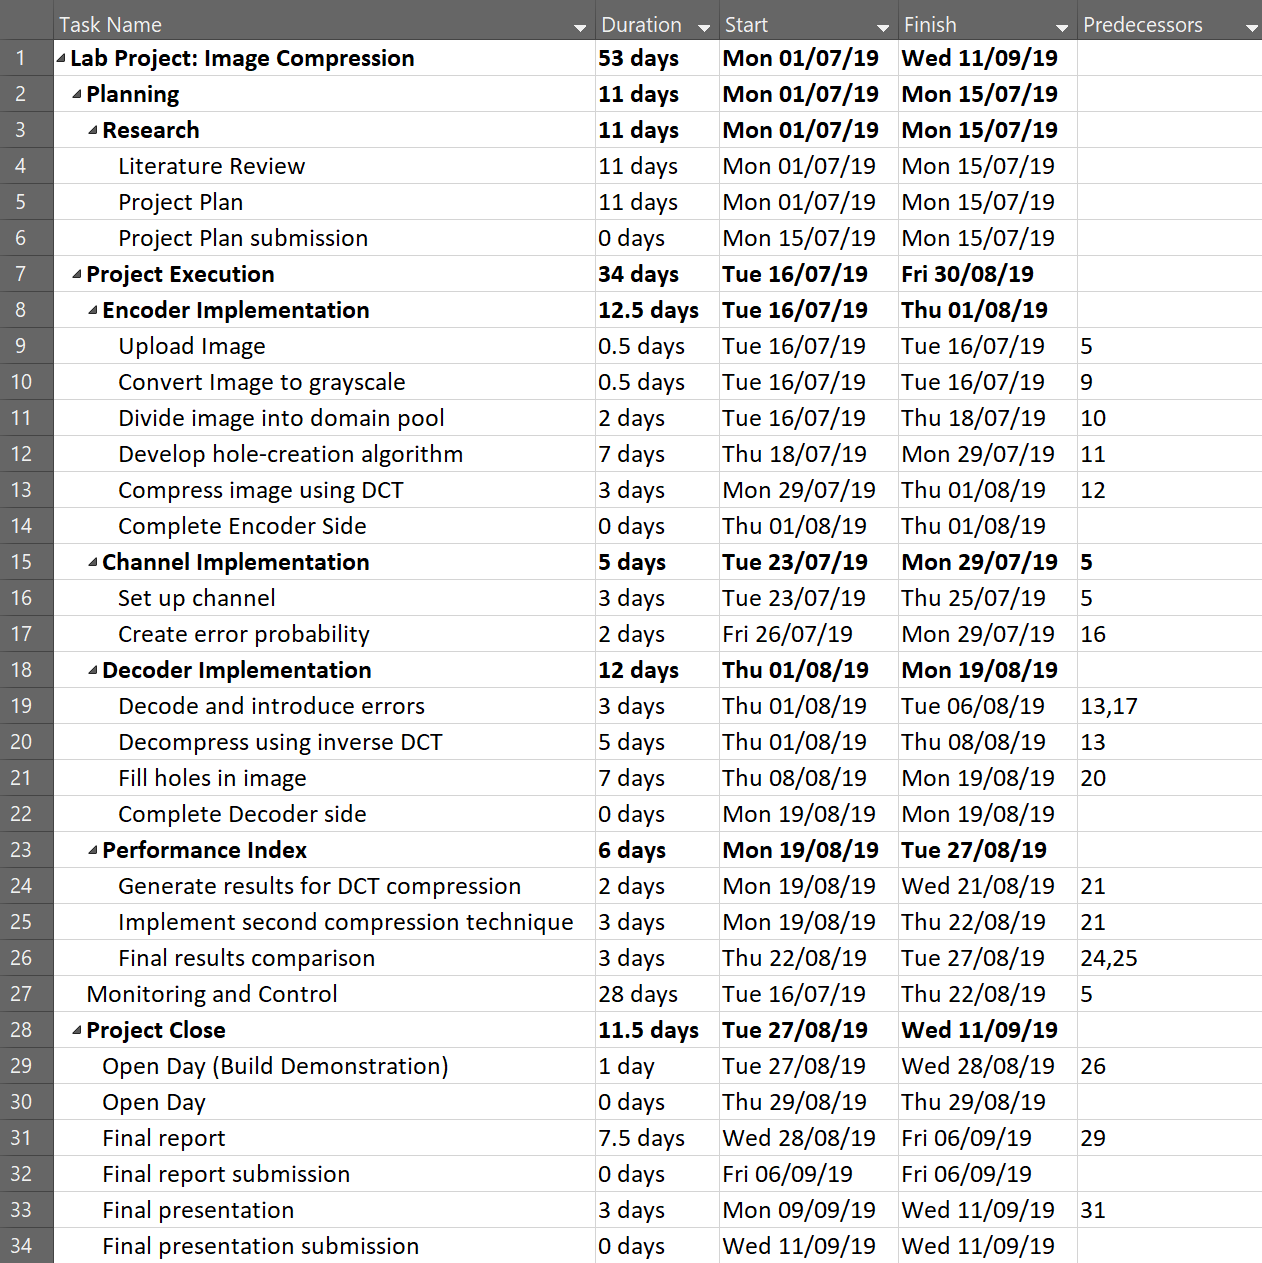
\includegraphics[scale=0.8, frame]{TableTasks.png}
\caption{Table showing the tasks and time allocated in completing the project}
\label{fig: Tasks}
\end{figure}

\newpage
\begin{landscape}
\begin{figure}[h!]
\renewcommand{\thefigure}{\arabic{figure}}
\centering
\hspace{-1.5cm}
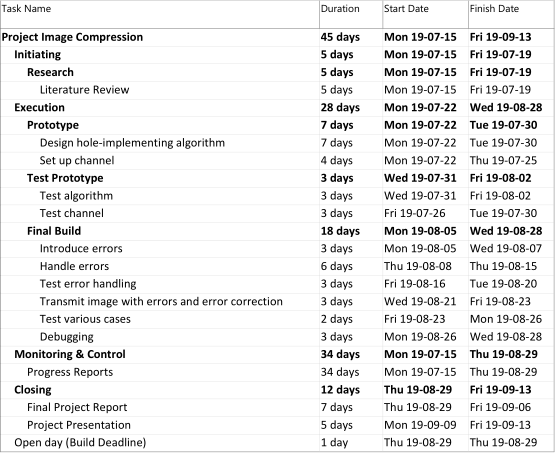
\includegraphics[scale=0.5, frame]{Gantt.png}
\caption{Gantt chart showing the tasks and time allocated in completing the project with the critical path highlighted}
\label{fig: Gantt}
\end{figure}
\end{landscape}

\end{document}

" vim: ts=4
" vim: tw=78
" vim: autoindent
" vim: shiftwidth=4
